\documentclass[12pt,a4paper]{article}

% Use Packages
\usepackage[polish]{babel}
\usepackage[T1]{fontenc}
\usepackage[letterpaper,top=2cm,bottom=2cm,left=3cm,right=3cm,marginparwidth=1.75cm]{geometry}
\usepackage{amsmath}
\usepackage{booktabs}
\usepackage{textcomp, gensymb}
\usepackage{graphicx}
\usepackage{float}
\usepackage{subcaption}
\usepackage{csquotes}
\usepackage{xurl}

%\usepackage[backend=bibtex,style=numeric]{biblatex}
%\addbibresource{bibliography.bib}

%font
\usepackage{tgtermes}

%Automatyczne linki w spisie treści
\usepackage[colorlinks=true, allcolors=blue]{hyperref}

% Set images path
\graphicspath{{./images/}}

\title{\huge{Model wykrywający anomalie w sygnałach EKG } }
\author{Bartosz Bizoń, Mateusz Grochowski, Filip Gnojek, Vladyslav Dikhtiaruk
\and \small{Opiekun pracy mgr. inż. Marek Lewiński}}
\date{Semestr VI \\ Rok akademicki 2023/2024}

\begin{document}

\pagenumbering{gobble}
\begin{figure}
    \begin{subfigure}{.49\textwidth}
      
\includegraphics[width=.7\linewidth]{images/PK_POZIOM_RGB.png}
      \centering
    \end{subfigure}
    \begin{subfigure}{.49\textwidth}
      
\includegraphics[width=.7\linewidth]{WM_RGB.png}
      \centering
    \end{subfigure}
\end{figure}
\maketitle


\begin{abstract} 
% W artykule przedstawiono przegląd modeli uczenia maszynowego służących do wykrywania anomalii w sygnałach EKG. Wykorzystano cztery modele: \textbf{LSTM} (z dokładnością identyfikacji anomalii na poziomie 72\%), \textbf{Gradient Boosting} (z dokładnością identyfikacji anomalii na poziomie 94\%), \textbf{XGBoosting} (z dokładnością identyfikacji anomalii na poziomie 98\%), \textbf{AdaBoosting} (z dokładnością identyfikacji anomalii na poziomie 87\%)
 %Skuteczność modeli została potwierdzona na zbiorze danych EKG pacjentów z różnymi schorzeniami sercowymi.

Celem niniejszej pracy było opracowanie i ocena różnych modeli do analizy danych EKG, w celu znalezienia najbardziej efektywnego narzędzia do ich przetwarzania i interpretacji. W celu znalezienia najlepszego rozwiązania, przeprowadziliśmy testy czterech modeli: LSTM, Gradient Boosting Classifier, XGBoost i AdaBoost. Model XGBoost osiągnął najwyższą dokładność na danych treningowych na poziomie 97\%, co jest dobrym wynikiem, ale może sugerować przetrenowanie. Ostatecznie po konsultacji z opiekunem pracy, zdecydowaliśmy, że model LSTM jest najodpowiedniejszy do dalszych prac, dzięki swojej zdolności do analizy szeregów czasowych. Model LSTM osiągał 73\% dokładności, ale wierzymy, że najlepiej sprawdził się w prawdziwych sytuacjach.

\end{abstract}

\newpage

\pagenumbering{arabic}
\tableofcontents

\newpage
\section{Wstęp}

\subsection{Waga problemu}
Choroby układu sercowo-naczyniowego stanowią najczęstszą przyczynę zgonów na świecie. W Polsce odpowiadają one za 37\% wszystkich zgonów, co oznacza, że co trzeci zgon jest spowodowany chorobą serca lub naczyń krążenia.

\subsection{Dane statystyczne}
Dane Polskiego Towarzystwa Kardiologicznego \cite{dane-o-problemach-z-sercem} są alarmujące: Ponad 10 milionów Polaków choruje na nadciśnienie tętnicze.
Co roku około 15 tysięcy osób umiera z powodu zawału serca.
Milion Polaków boryka się z niewydolnością serca, a liczba ta w ciągu dekady może wzrosnąć o połowę.
80 tysięcy Polaków rocznie doznaje zawału serca.
Prawie 2 miliony osób ma rozpoznaną chorobę niedokrwienną serca.
Około 1 milion 200 tysięcy osób cierpi na niewydolność serca.
600-800 tysięcy osób ma migotanie przedsionków.
Około 13 milionów Polaków ma nadciśnienie tętnicze, z czego część przypadków pozostaje nierozpoznana.
Prawie 20 milionów osób ma hipercholesterolemię.
8 milionów Polaków pali tytoń, co jest jednym z głównych czynników ryzyka chorób sercowo-naczyniowych.
Statystyki te pokazują ogrom skali problemu, jakim są choroby układu sercowo-naczyniowego w Polsce. Są one cichym zabójcą, który często nie daje wyraźnych objawów, a jego skutki mogą być tragiczne. Dlatego tak ważne jest profilaktyka i wczesne wykrywanie tych chorób. 

\subsection{EKG jako narzędzie diagnostyczne}
EKG, czyli elektrokardiogram, stanowi niezbędne narzędzie w diagnostyce chorób serca. Jest to zapis czynności elektrycznej serca, który pozwala na wykrycie wielu chorób sercowo-naczyniowych, takich jak zawały serca, arytmie i zaburzenia przewodzenia.

Tradycyjne metody analizy EKG opierają się na wizualnej ocenie zapisu przez wykwalifikowanego lekarza. Jednakże metoda ta jest czasochłonna i może być subiektywna, co może prowadzić do błędnych diagnoz. Z tego powodu istnieje potrzeba opracowania automatycznych systemów wykrywania anomalii w EKG, które mogą wspomagać pracę lekarzy i poprawić dokładność diagnostyki.


\section{Cel i zakres pracy}

\subsection{Cel}
Celem pracy jest prezentacja wybranych modeli oraz ocena ich skuteczności w wykrywaniu anomalii w EKG. Przeprowadzono badania na zbiorze danych zawierającym zapisy EKG pacjentów z różnymi chorobami sercowo-naczyniowymi oraz zdrowych osób. Wykorzystano wybrane algorytmy uczenia maszynowego, takie jak \textbf{LSTM}, \textbf{GradientBoostingClassifier}, \textbf{XGBoost}, \textbf{AdaBoost}. Dokonano oceny skuteczności każdego z modeli w zakresie identyfikacji anomalii w EKG i porównano je aby wyłonić model o najlepszych parametrach diagnostycznych. 

\subsection{Zakres pracy}
W niniejszej pracy zawarte zostały:
\begin{itemize}
    \item zapoznanie się z powagą problemu anomalii sercowych;
    \item przedstawienie definicji EKG;
    \item analiza anomalii występujących w EKG;
    \item omówienie metod klasyfikacyjnych i metod Boostingu;
    \item analiza zbioru danych;
    \item przeprowadzenie potoku OSEMN wykorzystując wybrane klasyfikatory; 
    \item ostateczna analiza wyników i sformułowanie wniosków końcowych. 
\end{itemize}




\section{Czym jest EKG?}

\subsection{Wprowadzenie}
Elektrokardiografia \textit{(eng. electrocardiography)} \cite{elektrokardiografia-wikipedia}  – zabieg diagnostyczny wykorzystywany w medycynie w celu oceny pracy serca i wykrycia ewentualnych jej zaburzeń.

Pomijając EKG wykonywane w czasie operacji na sercu, jest to metoda pośrednia polegająca na rejestracji elektrycznej czynności mięśnia sercowego z powierzchni klatki piersiowej w postaci różnicy potencjałów (napięć) pomiędzy dwiema elektrodami, co graficznie odczytujemy w formie krzywej elektrokardiograficznej, na specjalnym papierze milimetrowym bądź na ekranie monitora.

\begin{figure}[h]
    \centering
    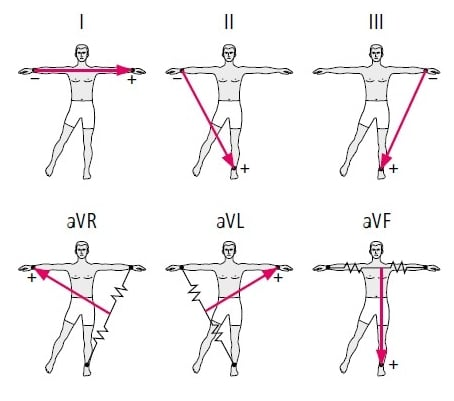
\includegraphics[width=0.75\linewidth]{images/ekg_odprowadzenia.jpg}
    \caption{Odprowadzenia kończynowe. \cite{ekg-odprowadzenia-konczynowe}}
\end{figure}

\subsection{Opis krzywej EKG}
Krzywa EKG, którą można zobaczyć na elektrokardiogramie, zbudowana jest z powtarzających się części. Jedna część (patrz ryc. 3.) odpowiada jednemu pełnemu cyklowi serca, od momentu napłynięcia krwi do przedsionków, poprzez skurcz przedsionków i komór, aż do momentu wypompowania krwi z serca. Interpretacja elektrokardiogramu jest trudna i wymaga doświadczenia, dlatego wynik badania EKG zawsze powinien odczytywać lekarz \cite{czym-jest-ekg-mp-pl}.

\begin{figure}[h]
    \centering
    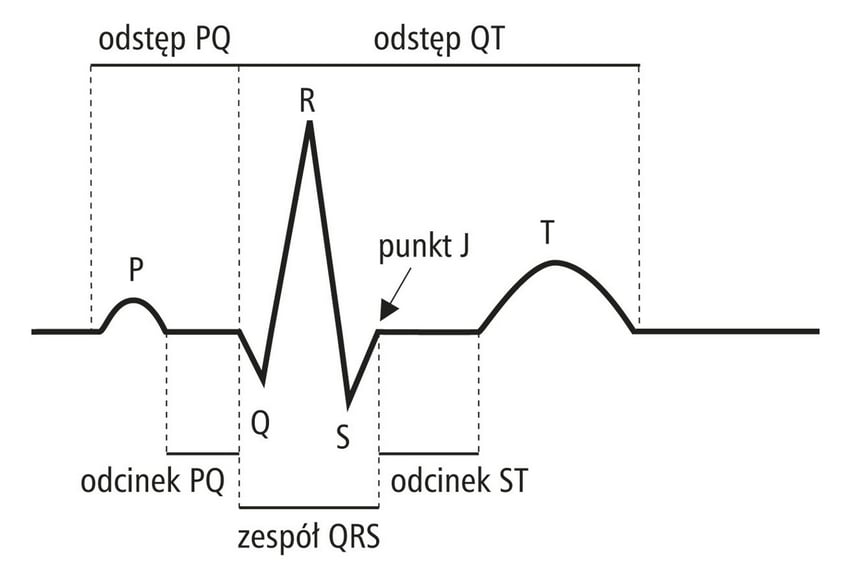
\includegraphics[width=0.75\linewidth]{images/krzywa-ekg.jpg}
    \caption{Krzywa EKG. \cite{ekg-analiza}}
\end{figure}

Załamek P powstaje w momencie skurczu przedsionków i przepompowania krwi do komór serca.
Zespół QRS przedstawia skurcz komór serca wypełnionych krwią.
Odcinki stanowią okres pomiędzy poszczególnymi fazami pracy serca, kiedy w sercu przekazywane jest pobudzenie.

\begin{figure}[H]
    \centering
    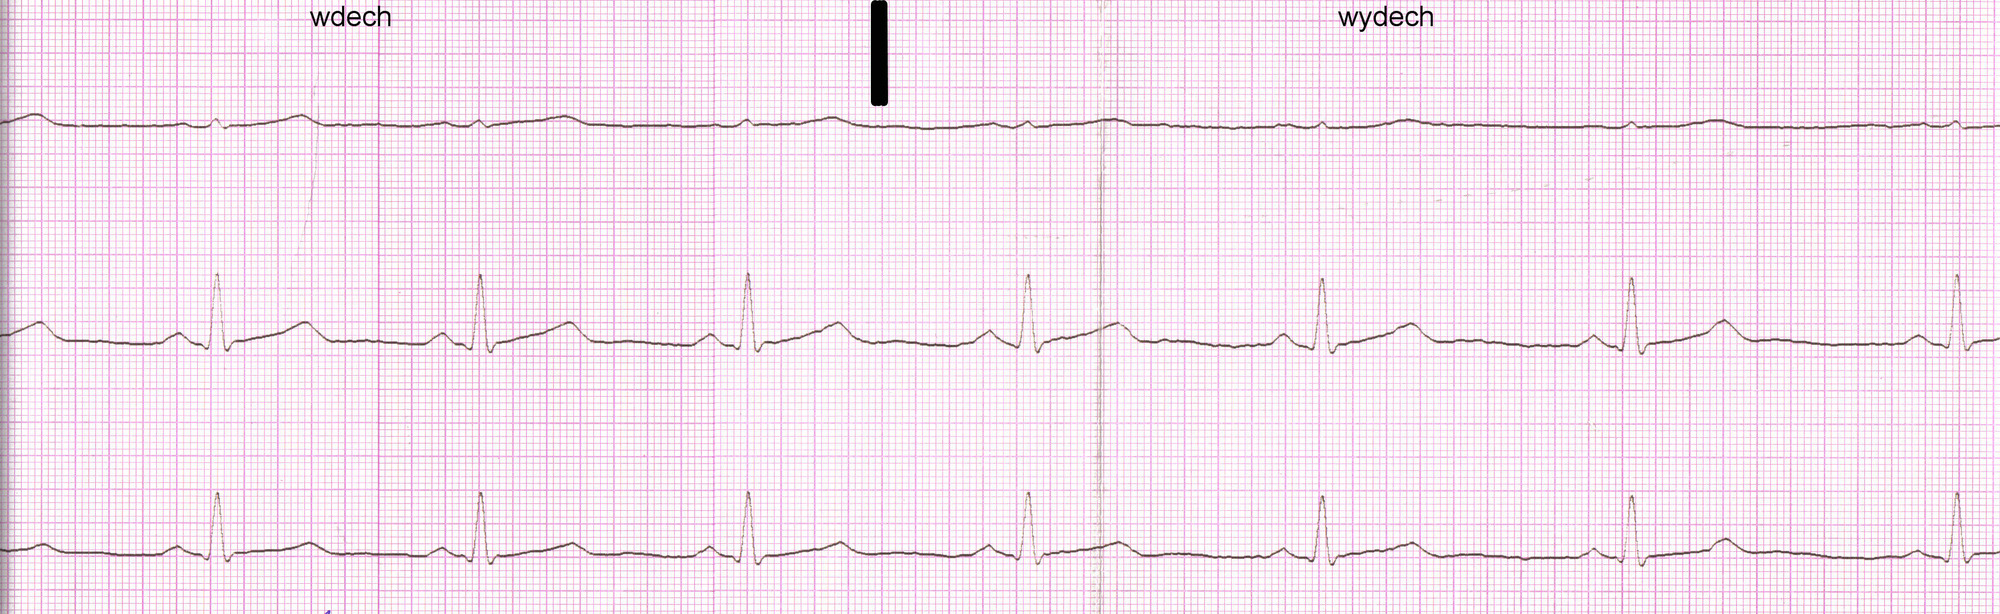
\includegraphics[width=1\linewidth]{EKG_wykres.jpg}
    \caption{Elektrokardiogram zdrowego, 21-letniego mężczyzny. Zaznaczony wdech i wydech. \cite{elektrokardiogram-wykres}}
\end{figure}

EKG nie jest niezawodnym kryterium rozpoznania choroby: istnieje możliwość prawidłowego elektrokardiogramu przy schorzeniach kardiologicznych oraz nieprawidłowy zapis czynności elektrycznej przy prawidłowym stanie klinicznym. 

\newpage{}

\section{Anomalie występujące w sygnałach EKG}
Istnieje wiele różnych rodzajów zaburzeń EKG \cite{ecg-abnormalities}, ale można je podzielić na dwie główne kategorie:

\subsection{Zaburzenia przewodzenia}
Zaburzenia przewodzenia \textit{(eng. Conduction Abnormalities)}.

\subsubsection{Blokady serca}
Blokady serca \textit{(eng. Heart Block)} to zaburzenia, które uniemożliwiają prawidłowy przepływ impulsów elektrycznych przez serce. Mogą być spowodowane uszkodzeniem układu przewodzenia lub zaburzeniami równowagi elektrolitowej. Istnieje trzy rodzaje blokad serca:
\begin{itemize}
    \item Blokady serca pierwszego stopnia - Te blokady powodują niewielkie spowolnienie przepływu impulsów elektrycznych przez serce. Zwykle nie powodują żadnych objawów.
    \item Blokady serca drugiego stopnia - Te blokady powodują bardziej znaczące spowolnienie przepływu impulsów elektrycznych przez serce. Mogą powodować objawy takie jak omdlenia, zawroty głowy i ból w klatce piersiowej.
    \item Blokady serca trzeciego stopnia - Te blokady uniemożliwiają przedostawanie się impulsów elektrycznych z przedsionków do komór. Mogą być śmiertelne, jeśli nie zostaną natychmiast wyleczone.
\end{itemize}

\subsubsection{Blokady odgałęzień pęczka}
Blokady odgałęzień pęczka \textit{(eng. Bundle Branch Block)} to zaburzenia, które uniemożliwiają prawidłowy przepływ impulsów elektrycznych przez komory. Mogą być spowodowane uszkodzeniem pęczka Hisa lub odgałęzień pęczka. Blokady odgałęzień pęczka mogą powodować objawy takie jak omdlenia, zawroty głowy i ból w klatce piersiowej.


\subsection{Zaburzenia rytmu serca}
Zaburzenia rytmu serca \textit{(eng. Rhythm Abnormalities)}.

\subsubsection{Arytmie nadkomorowe} 
Arytmie nadkomorowe to zaburzenia rytmu serca, które rozpoczynają się w przedsionkach. Mogą być spowodowane wieloma czynnikami, w tym chorobą serca, zaburzeniami równowagi elektrolitowej i lekami. Arytmie nadkomorowe mogą powodować objawy takie jak kołatanie serca, duszność i zmęczenie.

\subsubsection{Arytmie komorowe} 
Arytmie komorowe to zaburzenia rytmu serca, które rozpoczynają się w komorach. Mogą być spowodowane wieloma czynnikami, w tym chorobą serca, zaburzeniami równowagi elektrolitowej i lekami. Arytmie komorowe mogą być poważne, a nawet śmiertelne. Mogą powodować objawy takie jak kołatanie serca, omdlenia, a nawet nagły zgon sercowy.


\section{Metody, których możemy użyć w projekcie}
% Można wytrenować wiele różnych rodzajów algorytmów uczenia maszynowego w celu wykrywania anomalii \cite{anomaly-detection}. Do najpopularniejszych metod wykrywania anomalii należą:

% \subsection{Algorytmy oparte na gęstości}
% Algorytmy oparte na gęstości określają, kiedy wartość odstająca różni się od większego, a zatem gęstszego normalnego zestawu danych, przy użyciu algorytmów takich jak K-najbliższy sąsiad i las izolacyjny.

% \subsection{Algorytmy oparte na klastrach}
% Algorytmy oparte na klastrach oceniają, w jaki sposób dowolny punkt różni się od skupień powiązanych danych, przy użyciu technik takich jak analiza skupień K-średnich.

% \subsection{Algorytmy sieci Bayesa}
% Algorytmy sieci Bayesa opracowują modele służące do szacowania prawdopodobieństwa wystąpienia zdarzeń na podstawie powiązanych danych, a następnie identyfikowania znaczących odchyleń od tych przewidywań.

% \subsection{Algorytmy sieci neuronowych}
% Algorytmy sieci neuronowych uczą sieć neuronową przewidywania oczekiwanych szeregów czasowych, a następnie oznaczania odchyleń.

\subsection{Metody klasyfikujące}
W przypadku metod klasyfikujących \cite{Podrecznik-AI} w pierwszym kroku należy wspomnieć o definicji klasyfikacji. Klasyfikacja to przypisywanie pewnym próbkom przynależności do pewnych grup/klas. Dzielimy ją na następujące rodzaje:

\begin{itemize}
    \item \textbf{Binarna} - przewidywana wartość ma charakter dwuwartościowy(np. chory/zdrowy);
    \item \textbf{Wieloklasowa} - przewidywana wartość może należeć do jednej z wielu klas (np. "zielony", "czerwony" lub "niebieski");
    \item \textbf{Wieloetykietowa} - przewidywana wartość dotyczy wielu zmiennych jednocześnie (np. "drogi czerwony samochód") 
\end{itemize}

\paragraph{Wśród najpopularniejszych modeli klasyfikujących wyróżnić można:}

\subsubsection{Regresja Liniowa} 
Regresja logistyczna, mimo że w nazwie ma słowo \textit{regresja}, jest używana do rozwiązywania problemów klasyfikacji binarnej, czyli takich, gdzie dane mogą należeć tylko do jednej z dwóch kategorii. Jest to prosta metoda klasyfikacji, często używana jako pierwszy krok, aby stworzyć podstawowy model przed zastosowaniem bardziej skomplikowanych technik. W regresji logistycznej używa się liniowego połączenia różnych zmiennych, aby oszacować prawdopodobieństwo, że wynik będzie 0 lub 1. To właśnie dlatego w nazwie jest słowo "regresja". Ponieważ prawdopodobieństwo oblicza się na podstawie liniowej kombinacji zmiennych, modele regresji logistycznej są łatwe do interpretacji.

\begin{figure}[h]
    \centering
    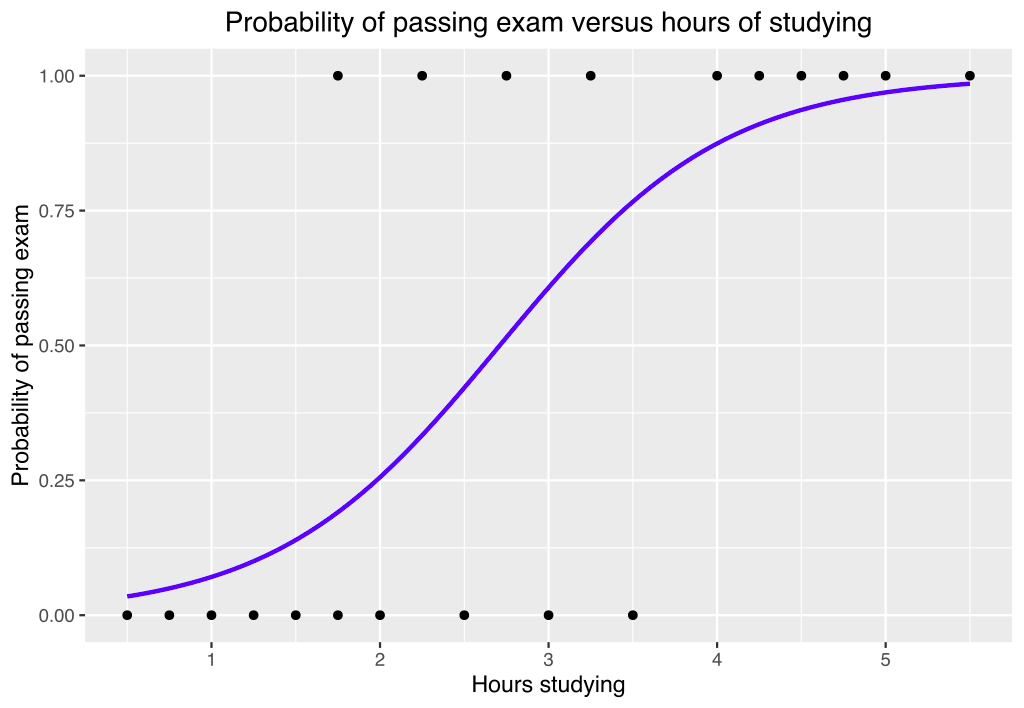
\includegraphics[width=0.75\linewidth]{images/ligistic-curve.png}
    \caption{Przykładowy wykres regresji logistycznej \cite{logistic-regression-graph}}
\end{figure}

\subsubsection{Metoda K najbliższych sąsiadów} 
Algorytm k najbliższych sąsiadów \textit{(eng. k-nearest neighbor)} (KNN) klasyfikuje punkty danych na podstawie ich odległości do innych punktów w zbiorze treningowym. Najpierw dane treningowe są ładowane do modelu, a gdy pojawia się nowa próbka do sklasyfikowania, model szuka najbliższych k sąsiadów tej próbki. Jeśli k wynosi 5, model znajdzie pięciu najbliższych sąsiadów i przeprowadzi głosowanie, aby przypisać etykietę nowej próbce. W przypadku regresji model oblicza średnią wartość k najbliższych sąsiadów. Czas odpowiedzi może być dłuższy przy dużej liczbie danych, ponieważ model musi przeszukiwać cały zbiór danych. KNN może być również mylony przez nieistotne atrybuty, co można poprawić, przypisując wagi do danych.

\subsubsection{Naiwny klasyfikator Bayesa} 
Algorytm naiwnego Bayesa jest techniką klasyfikacji, która zakłada, że każda cecha jest niezależna od innych. Podczas trenowania modelu oblicza prawdopodobieństwa dla każdej klasy oraz prawdopodobieństwa warunkowe dla każdej cechy w odniesieniu do danej klasy. Następnie wykorzystuje twierdzenie Bayesa, aby określić prawdopodobieństwo, że dane wejściowe należą do określonej klasy na podstawie zaobserwowanych cech. Po obliczeniu tych prawdopodobieństw, algorytm przypisuje dane wejściowe do klasy z najwyższym prawdopodobieństwem. Dzięki swojej prostocie, algorytm jest szybki w trenowaniu i klasyfikacji, co czyni go wydajnym nawet przy ograniczonych zasobach CPU i pamięci. Ponadto dobrze radzi sobie z ciągłymi aktualizacjami, co oznacza, że może być łatwo dostosowywany do nowych danych bez konieczności trenowania od nowa całego modelu. Przykładowo, w filtrach spamu analizuje cechy wiadomości e-mail, aby ocenić, czy dana wiadomość jest spamem.

\subsubsection{Drzewa Decyzyjne} 
Decyzyjne drzewa są narzędziem analizy danych, które przewidują odpowiedzi na podstawie serii decyzji podejmowanych na różnych etapach. Drzewa klasyfikacyjne dostarczają odpowiedzi nominalne, takie jak prawda lub fałsz, podczas gdy drzewa regresyjne generują wartości numeryczne. Są względnie łatwe do zrozumienia, umożliwiając śledzenie ścieżki od korzenia do liścia. Jest to szczególnie przydatne, gdy potrzebujemy wyjaśnić wyniki osobom zainteresowanym procesem podejmowania decyzji. Jednak główną wadą decyzyjnych drzew jest tendencja do nadmiernego dopasowania, choć istnieją metody ensemble, które temu przeciwdziałają. 

\subsubsection{Maszyna wektorów nośnych} 
Maszyna wektorów nośnych (SVM) używana jest, gdy dane posiadają dokładnie dwie klasy. Działa poprzez klasyfikację danych, znajdując najlepszą hiperpłaszczyznę, która oddziela punkty jednej klasy od punktów drugiej klasy (najlepsza hiperpłaszczyzna to ta z największym marginesem między klasami). W przypadku więcej niż dwóch klas, SVM tworzy zestaw podproblemów klasyfikacji binarnej (z jednym uczniem SVM dla każdego podproblemu). SVM posiada kilka mocnych stron. Jest niezwykle dokładny i unika nadmiernego dopasowania danych. Liniowe maszyny wektorów nośnych są stosunkowo łatwe do interpretacji. Po przeszkoleniu, modele SVM są bardzo szybkie, a dane treningowe można usunąć, jeśli jest ograniczona dostępna pamięć.

\begin{figure}[h]
    \centering
    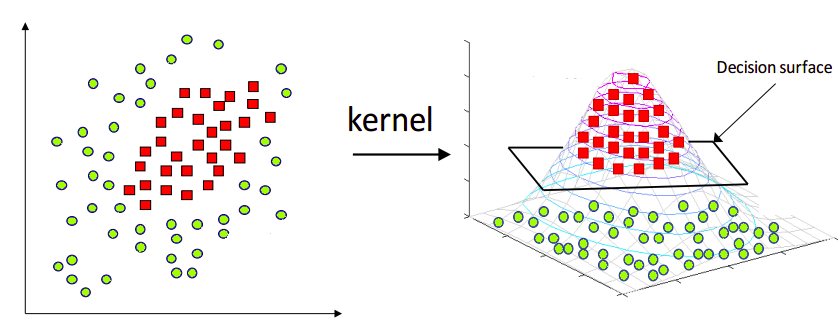
\includegraphics[width=0.75\linewidth]{images/svm-visualization.png}
    \caption{Wizualizacja działania SVM \cite{svm-visualization}}
\end{figure}

\subsubsection{Sieci Neuronowe}
Sztuczne sieci neuronowe (ANN) uczą się i są trenowane do rozwiązywania problemów, rozpoznawania wzorców oraz przewidywania zdarzeń. Ich zachowanie jest determinowane przez połączenia między poszczególnymi elementami obliczeniowymi oraz ich siłę, czyli wagi, które są dostosowywane automatycznie w trakcie treningu. Dla zaawansowanych użytkowników ANN są przydatne do modelowania danych nieliniowych z dużą liczbą cech wejściowych. Mimo to, sieci neuronowe są kosztowne obliczeniowo, trudne do zrozumienia i dostrojenie ich często nie jest praktyczne. \cite{classification-models}

\subsection{Boosting}
\label{sec:boosting}
Boosting to technika algorytmu uczenia maszynowego, która polega na łączeniu słabych modeli w mocny model. 
W boostingu, wybierana jest losowa próbka danych, dopasowywana do modelu, a następnie trenowana sekwencyjnie.
Podczas każdej iteracji, słabe reguły z klasyfikatorów są łączone, formując jedną silną. Używanie wzmacniania może poprawić precyzyjność predykcji wytrenowanego modelu.  \cite{boosting-1}


Boosting jest iteracyjną metodą, w której każdy kolejny model uczy się na zmodyfikowanej wersji zbioru treningowego. W tej modyfikacji, przykładom błędnie klasyfikowanym przez poprzednie modele przypisywana jest wyższa waga. Chodzi o to, aby skupić się na przykładach, które były trudne do klasyfikacji przez poprzednie modele i wymusić na kolejnych modelach poświęcenie im większej uwagi. W ten sposób kolejne modele mogą uczyć się na błędach poprzednich i poprawiać ogólną wydajność całego modelu. Należy jednak pamiętać, że boosting może również prowadzić do przeuczenia, jeśli modele będą zbyt skomplikowane lub jeśli zestaw danych będzie zbyt mały. \cite{boosting-2} 

\begin{figure}[H]
    \centering
    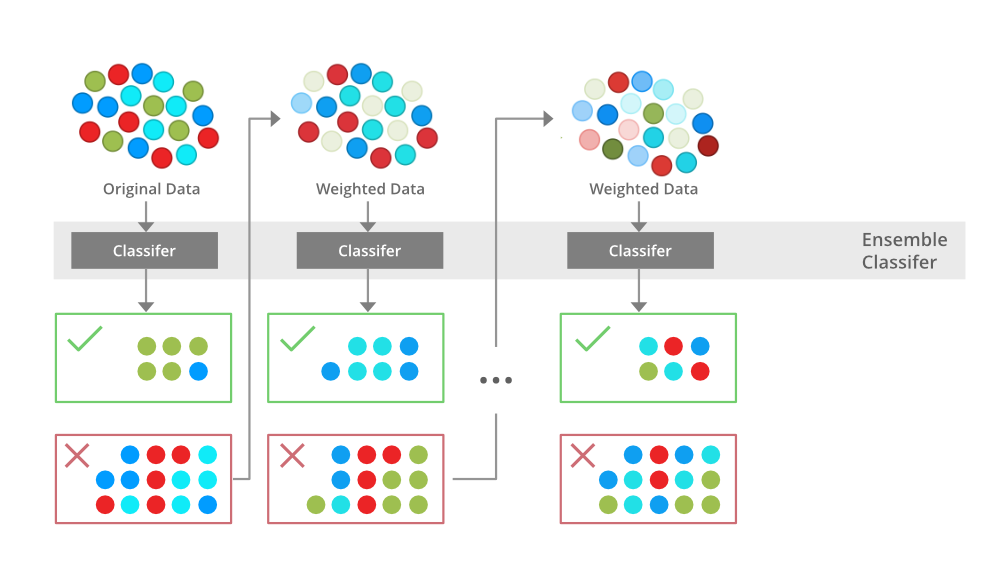
\includegraphics[width=1\linewidth]{images/boosting-diagram.png}
    \caption{Diagram działania modeli boostujących \cite{boosting-diagram}}
\end{figure}

\subsubsection{Gradient Boosting}
\label{sec:gradient-boosting}

Gradient Boosting to nadzorowany algorytm uczenia maszynowego stosowany w klasyfikacji i regresji. Jest to technika zespołowa, która wykorzystuje wiele słabych modeli do stworzenia silnego modelu dla regresji i klasyfikacji. \cite{gradient-boosting}


Gradient boosting opiera się na trzech kluczowych elementach:
\begin{itemize}
 \item \textbf{Funkcja strat} \textit{(ang. loss function)} -  miara błędu popełnianego przez model. Algorytm gradient boostingu stara się zminimalizować tę funkcję, aby poprawić ogólną wydajność modelu.
 
 \item \textbf{Słaby uczący się} \textit{(ang. weak learner)} - prosty model, taki jak pojedyncze drzewo decyzyjne. Słabe uczące się są łączone w celu stworzenia silniejszego modelu.
 
 \item \textbf{Model addytywny} - sposób na łączenie słabych uczących się. Każdy kolejny słaby uczący się jest dodawany do modelu w celu skorygowania błędów popełnionych przez poprzednie modele, co prowadzi do minimalizacji funkcji strat.
\end{itemize}

\subsubsection{XGBoosting}
\label{sec:xgboosting}
XGBoost \textit{(eng. Extreme Gradient Boosting)} \cite{xg-boost} to algorytm gradientnego boostingu wykorzystujący drzewa decyzyjne jako słabe modele. Działa on poprzez iteracyjne uczenie drzew decyzyjnych w celu korygowania błędów popełnionych przez poprzednie drzewa. Celem jest minimalizacja funkcji strat.

\subsubsection{AdaBoost}
\label{sec:adaboosting}
AdaBoost \textit{(eng. Adaptive boosting)} to jeden z pierwszych opracowanych algorytmów gradientnego boostingu. Jest on głównie wykorzystywany do zadań klasyfikacji, a bazowy uczący się (algorytm uczenia maszynowego, który jest wzmacniany) to zwykle drzewo decyzyjne z tylko jednym poziomem, nazywane również \textit{(ang. decision stump)}. \cite{adaboost}

Algorytm ten wykorzystuje ważone błędy, aby zbudować silny klasyfikator z serii słabych klasyfikatorów. Działa to w następujący sposób:
\begin{itemize}
    \item Wagi dla każdej próbki danych są początkowo równe.
    \item Trenowany jest słaby klasyfikator (np. "decision stump").
    \item Analizowane są błędy klasyfikatora. Próbkom błędnie sklasyfikowanym przypisywana jest większa waga.
    \item Proces powtarzany jest iteracyjnie, przy czym każdy nowy słaby klasyfikator skupia się na próbkach, które poprzednie modele klasyfikowały błędnie.
    \item Ostateczny wynik klasyfikacji uzyskiwany jest przez ważoną kombinację wszystkich słabych klasyfikatorów.
\end{itemize}



\section{Zbiór danych wybrany do projektu}

\subsection{Oryginalny zbiór}
Oryginalny zbiór danych \cite{ptb-diagnostic-ecg-database} zawiera zapisy EKG uzyskane przy użyciu niekomercyjnego prototypowego rejestratora PTB o następujących parametrach technicznych:
\begin{itemize}
    \item 16 kanałów wejściowych (14 dla EKG, 1 dla oddechu, 1 dla napięcia sieciowego)
    \item Napięcie wejściowe: ± 16 mV, kompensowane napięcie offsetu do ± 300 mV
    \item Rezystancja wejściowa: 100 $\Omega$ (DC)
    \item Rozdzielczość: 16 bitów z 0,5 \micro V/LSB (2000 jednostek A/C na mV)
    \item Pasmo przenoszenia: 0 - 1 kHz (synchronizacja próbkowania wszystkich kanałów)
    \item Napięcie szumu: maks. 10 \micro V (pp), odpowiednio 3 \micro V (RMS) przy zwarciu wejściowym
    \item Pomiar online rezystancji skóry
    \item Pomiar poziomu szumu podczas zbierania sygnału
\end{itemize}

Baza danych zawiera 549 zapisów od 290 osób (w wieku od 17 do 87 lat, średnio 57,2; 209 mężczyzn, średni wiek 55,5 i 81 kobiet, średni wiek 61,6; wiek nie został zarejestrowany dla 1 kobiety i 14 mężczyzn). Każda osoba jest reprezentowana przez jeden do pięciu zapisów. Brak osób o numerach 124, 132, 134 i 161. Każdy zapis zawiera 15 jednocześnie mierzonych sygnałów: 12 standardowych odprowadzeń (i, ii, iii, avr, avl, avf, v1, v2, v3, v4, v5, v6) wraz z 3 odprowadzeniami EKG w układzie Franka (vx, vy, vz). Każdy sygnał jest digitalizowany z częstotliwością 1000 próbek na sekundę, z rozdzielczością 16 bitów w zakresie ± 16,384 mV. Na specjalne życzenie udostępniających bazę danych, nagrania mogą być dostępne z częstotliwością próbkowania do 10 kHz.

W pliku nagłówkowym (.hea) większości tych zapisów EKG znajduje się szczegółowe podsumowanie kliniczne, w tym wiek, płeć, diagnoza, a jeśli dotyczy, dane dotyczące historii choroby, leków i interwencji, patologii tętnic wieńcowych, wentrikulografii, echokardiografii i hemodynamiki. Podsumowanie kliniczne nie jest dostępne dla 22 osób. Klasy diagnostyczne pozostałych 268 osób podsumowano poniżej.

\subsection{Klasy diagnostyczne anomalii występujących we zbiorze}

\begin{table}[H]
    \centering
    \begin{tabular}{|c|c|}
         \hline
         \textbf{Klasa diagnostyczna} & \textbf{Ilość przypadków} \\
         \hline
         Zawał mięśnia sercowego & 148 \\ 
         \hline
         Kardiomiopatia/niewydolność serca & 18 \\
         \hline
         Blok odnogi pęczka Hisa & 15 \\
         \hline
         Arytmia & 14 \\
         \hline
         Przerost mięśnia sercowego & 7 \\
         \hline
         Wada zastawkowa serca & 6 \\
         \hline
         Zapalenie mięśnia sercowego & 4 \\
         \hline
         Różne choroby serca & 4 \\
         \hline
         Kontrole zdrowia & 52 \\
         \hline
    \end{tabular}
    \caption{Podsumowanie klas diagnostycznych występujących we zbiorze.}
    \label{tab:anomalies_in_dataset}
\end{table}

\subsection{Forma zbioru danych w jakiej go importujemy}
Zestaw danych wybrany do projektu pochodzi ze zbioru \textit{"The PTB Diagnostic ECG Database"} opisanego powyżej, którego poddano obróbce \cite{ecg-heartbeat-categorization-dataset}. Sygnały zawarte we zbiorze odpowiadają kształtom elektrokardiogramu (EKG) dla osób zdrowych oraz dla osób dotkniętych różnymi chorobami, w ten sposób oryginalny zbiór uproszczony jest do dwóch kategorii (sygnały normalne oraz anomalie). Autor kaggle podzielił dane według tych kategorii na dwa pliki \textit{"ptbdb\_normal.csv"} z danymi osób zdrowych i \textit{"ptbdb\_abnormal.csv"} z danymi osób cierpiących na różne choroby serca. Sygnały te są wstępnie przetworzone i segmentowane, przy czym każdy segment odpowiada uderzeniu serca.

Gotowy zbór zawiera \textbf{14552 próbek}, częstotliwość próbkowania danych to \textbf{125Hz}. Wszystkie próbki były przycinane, próbkowane w dół i uzupełniane zerami, jeśli było to konieczne, do \textbf{wymiaru 188}.


\section{Rozpoczęcie potoku OSEMN}
\begin{figure}[h]
    \centering
    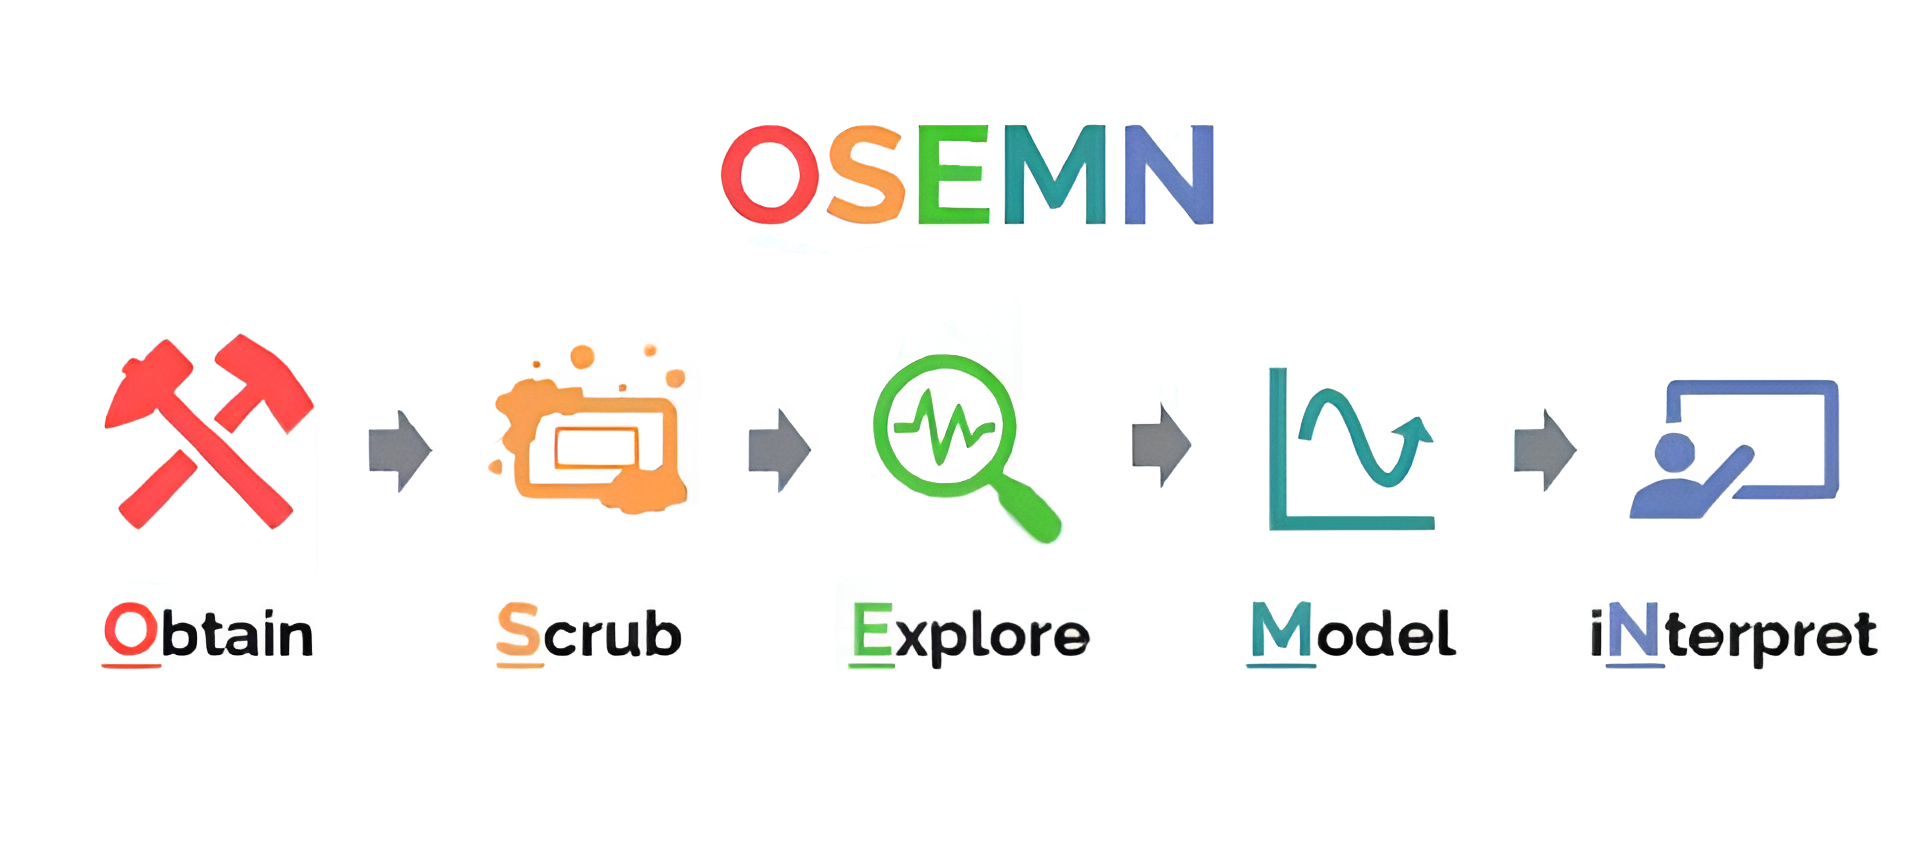
\includegraphics[width=1\linewidth]{images/osemn.png}
    \caption{Diagram potoku OSEMN i znaczenie po angielsku \cite{osemn}}
\end{figure}

\subsection{Import danych}
Zaimportowane dane mają \textbf{188} kolumn oraz \textbf{4046} wierszy dla danych "normal" i \textbf{10506} dla danych "abnormal". Łącznie daje nam to \textbf{14552 wierszy} danych. Dysproporcja pomiędzy danymi normalnymi i danymi z anomaliami trochę nas martwi, decydujemy się jednak kontynuować.

\subsection{Spojrzenie na dane}
W tabeli \ref{tab:dane_po_imporcie} pokazano wygląd danych po imporcie. Są to po prostu wartości poszczegółnych pomiarów na wykresie EGK, a każdy z wierszy to segment, czyli część wykresu EKG zawierająca dokładnie \textbf{188 pomiarów}. Wartości te zostały \textbf{znormalizowane od 0 do 1}. Można także zauważyć, iż pierwsza kolumna to najprawdopodobniej pik na wykresie EKG, od którego zaczyna się każdy z segmentów danych. Poniżej przedstawiono także wykresy \ref{fig:pierwszy-wiersz-normal} oraz \ref{fig:pierwszy-wiersz-abnormal} obrazujące pierwsze z wierszy w kolejno danych "normal" i "abnormal".

\begin{table}[H]
    \centering
    \begin{tabular}{|l|l|l|l|l|l|l|l|l|}
    \hline
        0 & 1.000000 & 0.900324 & 0.358590 & 0.051459 & 0.046596 & 0.126823 & 0.133306 & 0.119125 \\ \hline
        1 & 1.000000 & 0.794681 & 0.375387 & 0.116883 & 0.000000 & 0.171923 & 0.283859 & 0.293754 \\ \hline
        2 & 0.909029 & 0.791482 & 0.423169 & 0.186712 & 0.000000 & 0.007836 & 0.063032 & 0.077002 \\ \hline
        3 & 1.000000 & 0.478893 & 0.056760 & 0.064176 & 0.081289 & 0.072732 & 0.055619 & 0.048774 \\ \hline
        4 & 1.000000 & 0.867238 & 0.201360 & 0.099349 & 0.141336 & 0.120934 & 0.108516 & 0.096393 \\ \hline
        5 & 0.948983 & 0.505265 & 0.004176 & 0.022513 & 0.059550 & 0.107298 & 0.110385 & 0.111293 \\ \hline
        6 & 1.000000 & 0.487680 & 0.114305 & 0.000000 & 0.030116 & 0.065024 & 0.060917 & 0.050992 \\ \hline
        7 & 1.000000 & 0.460381 & 0.122178 & 0.009296 & 0.125719 & 0.220009 & 0.267375 & 0.262948 \\ \hline
        8 & 1.000000 & 0.755102 & 0.135116 & 0.000000 & 0.285714 & 0.331457 & 0.256861 & 0.258269 \\ \hline
        9 & 1.000000 & 0.706176 & 0.323144 & 0.101684 & 0.013724 & 0.222707 & 0.285714 & 0.295696 \\ \hline
    \end{tabular}
    \caption{Wygląd danych po imporcie.}
    \label{tab:dane_po_imporcie}
\end{table}

\begin{figure}[h]
    \centering
    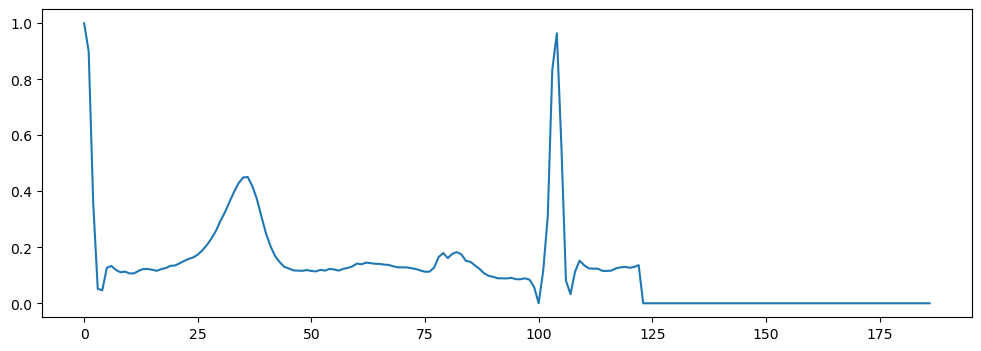
\includegraphics[width=1\linewidth]{pierwszy_wiersz_normal.png}
    \caption{Pierwszy z wierszy w danych "normal"}
    \label{fig:pierwszy-wiersz-normal}
\end{figure}

\begin{figure}[h]
    \centering
    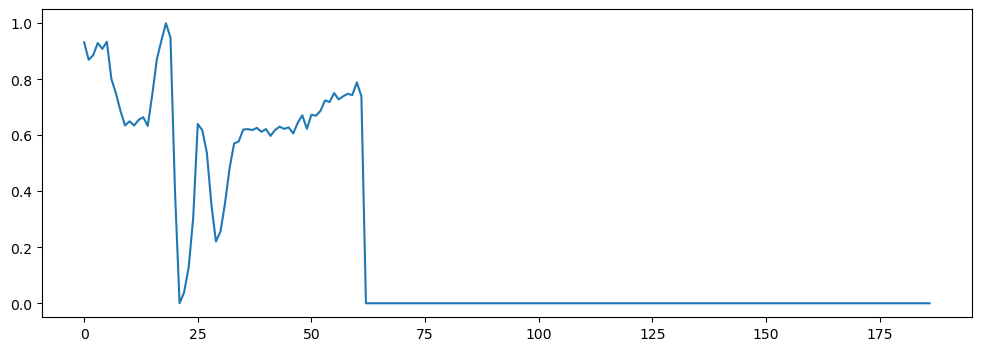
\includegraphics[width=1\linewidth]{pierwszy_wiersz_abnormal.png}
    \caption{Pierwszy wiersz w danych "abnormal"}
    \label{fig:pierwszy-wiersz-abnormal}
\end{figure}


\section{Preprocessing}
\subsection{Wstępna obróbka}

Zauważyliśmy, że w danych występują wartości \textbf{NaN}, które mogłyby przeszkodzić w dalszej pracy z danymi. Postanowiliśmy je więc usunąć ze zbioru. Rozwiązanie to wydawało się rozsądne, ponieważ wartości tych nie było dużo.

Drugim krokiem, który podjęliśmy było usunięcie kolumny z oznaczeniem klasy (0 dla danych normalnych i 1 dla danych z anomaliami). Kolumna ta mogłaby zaburzyć filtrowanie, które zamierzamy przeprowadzić. 

Filtrowanie zdecydowaliśmy się zastosować na danych w celu usunięcia niepotrzebnych szumów, które mogłyby przeszkodzić w uczeniu modeli. Przeprowadziliśmy je przy użyciu biblioteki \textbf{HeartPy} opisanej w sekcji \ref{sec:heartpy}. Więcej szczegółów na temat filtrowania opisano także w sekcji \ref{sec:filtrowanie}.

\subsection{Biblioteka HeartPy} \label{sec:heartpy}
\textbf{HeartPy} \cite{heartpy-1,heartpy-2}, czyli zestaw narzędzi do analizy tętna w Pythonie, to moduł służący do analizy rytmu serca w języku Python. Powstał jako implementacja pythonowa do analizy danych fizjologicznych, zbieranych w naturalnych eksperymentach podczas jazdy samochodem i na rowerze.

Moduł przyjmuje sygnał tętna i zwraca pomiary w domenie czasu i częstotliwości, często spotykane w literaturze naukowej. Posiada ona również filtry, które poprawią jakość danych.

W naszym projekcie postanowiliśmy użyć tej biblioteki do filtrowania danych.

\subsection{Filtrowanie sygnału za pomocą biblioteki Heartpy} \label{sec:filtrowanie}
Dzięki bibliotece Heartpy jesteśmy w stanie przygotować sygnał pobrany z urządzeń. Sygnał nieobrobiony zawiera wiele szumów co negatywnie wpływa na wykrywanie cech z sygnału. Biblioteka Heartpy również jest zaopatrzona w odpowiednie filtry dzięki czemu możemy przygotować sygnał do dalszego przetwarzania.

\begin{figure}[H]
    \centering
    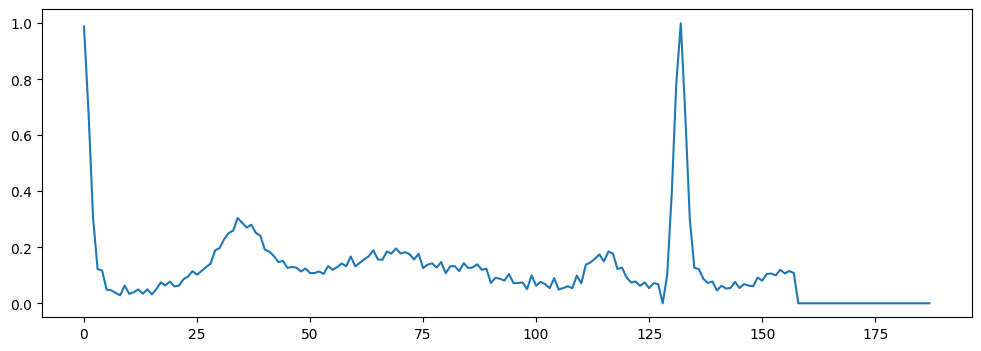
\includegraphics[width=1\linewidth]{heartpy-nofilter.png}
    \caption{Wykres sygnału przed filtracją}
\end{figure}

\begin{figure}[H]
    \centering
    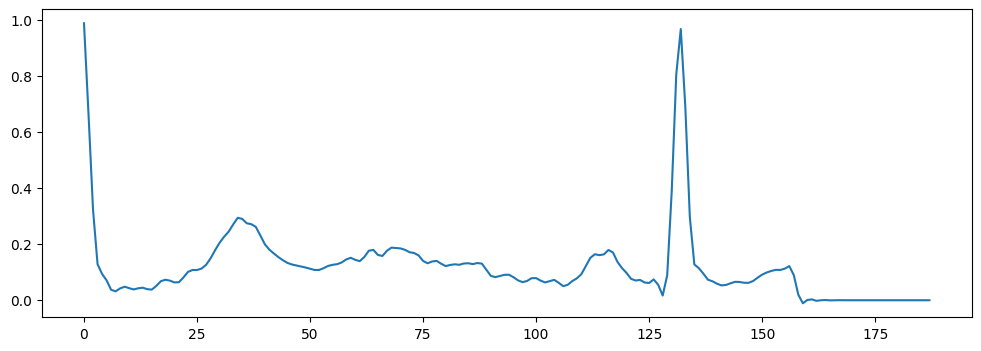
\includegraphics[width=1\linewidth]{images/heartpy-filter.png}
    \caption{Wykres sygnału po filtracji dolnoprzepustowej}
\end{figure}

\subsection{Podział na zbiory uczące i testowe}
Dlatego, że nasz zbiór znajdował się w dwóch plikach i importowaliśmy go osobno, museliśmy go połączyć. W tym celu do każdego ze zbiorów dodaliśmy kolumnę oznaczającą klasę. Jak wcześniej wspominaliśmy: \textbf{0 dla klasy normal} i \textbf{1 dla klasy abnormal}. Dzięki czemu mogliśmy połączyć te zbiory bez utraty informacji o klasie.

Następnie w standardowy sposób podzieliliśmy dane na uczące i testowe. Postanowiliśmy, że podział ten będzie w propocjach \textbf{75\% dla zbioru uczącego i 25\% dla zbioru testowego}.

\section{Przygotowanie, trenowanie i testowanie modeli}
Dla porównania sprawności modeli użyliśmy paru popularnych modeli klasyfikacyjnych oraz rekurencyjne sieci neuronowej.

\subsection{LSTM}
LSTM, czyli typ rekurencyjnych sieci neuronowych dobrze się nadaję do analizy przebiegów czasowych, czyli w naszym przypadku danych z EKG.

Dane trzeba było zreshapować aby można było ich użyć do modelu. Po 10 epokach trenowania model osiągnął 72.29\% dokładności, co nie jest najlepszym wynikiem, ale uważamy, że można ten wynik poprawić, i że ta ścieżka i te modele byłyby lepsze, ponieważ lepiej sprawdzałyby się w warunkach produkcyjnych.

\subsection{Gradient Boosting}
Podstawowy klasyfikator, którego użyliśmy w projekcie to zawarty w bibliotece Scikit learn Gradient Boost, czyli metoda zespołowa z wykorzystaniem boostingu opisanego lepiej w sekcji \ref{sec:boosting} i \ref{sec:gradient-boosting}.

Model został wytrenowany przy pomocy sprawdzianu krzyżowego \textit{(eng. cross validation)} trenując 10 modeli z różnymi parametrami. Modele osiągnęły dokładność na poziomie 91.77\% i odchylenie standardowe na poziomie 0.78 co jest całkiem niezłym wynikiem, a odchylenie standardowe wskazuje, że parametry nie mają dużego wpływu na ten model. 

\subsection{XGBoosting}
Drugi klasyfikator jakiego użyliśmy to XGBoost \textit{(eng. Extreme Gradient Boosting)} \cite{xg-boost}, o którym możemy więcej poczytać w sekcji \ref{sec:xgboosting}.

Klasyfikator również wytrenowaliśmy przy użyciu cross validation. I ten model osiągnął lepsze wyniki bo przy 10 modelach średnia dokładność to aż 97.48\%, a odchylenie standardowe wyniosło 0.48. 

\subsection{AdaBoosting}
Trzeci klasyfikator to AdaBoost o którym możemy więcej poczytać w sekcji \ref{sec:adaboosting}

Klasyfikator przy użyciu sprawdzianu krzyżowego osiągnął dokładność na poziomie 86.41\% i odchylenie standardowe na poziomie 0.61, co pokazuje, że w przypadku tego zadania radzi on sobie gorzej niż inne klasyfikatory użyte w tej pracy.

\section{Wnioski}

% - Znaleźliśmy podobny projekt na Medium, ale po jego analizie okazało się że jest zupełnie błędny. Dane były źle zinterpretowane, wyniki uzyskane z heartpy w tym artykule były absolutnie niesprawdzowne i błędne ("normalne" tętno na poziomie 600 BPM) oraz źle dobrany model do zagadnienia

% - Próbowaliśmy to zrobić z heartpy, ale okazało się, że moduł wyciągający informacje z danych EKG w tej bibliotece nie jest przeznaczony do danych w takiej postacji w jakiej mieliśmy - wyciągał błędne wnioski, na przykład BPM wynosiło 500 lub 1000, co jest niemożliwe.

% - Opisać najlepszy model z wybranych przez nas (XGBoost, AdaBoost, Gradient Boost z Scikit Learn, LSTM z tensorflow) Wyniki modeli:
% Dokładność LSTM na danych treningowych: 72.05%.
% Dokładność LSTM na danych testowych: 72.29%.
% Dokładność Gradient Boosting Classifier na danych treningowych: 94.76%.
% Dokładność Gradient Boosting Classifier na danych testowych: 93.54%.
% Dokładność XGBoost na danych treningowych: 100.00%.
% Dokładność XGBoost na danych testowych: 97.80%.
% Dokładność AdaBoost na danych treningowych: 88.33%.
% Dokładność AdaBoost na danych testowych: 87.30%.


% - Mimo że XGBoost ma teoretycznie najlepszy wynik (oznacza to najprawdopodobniej przetrenowanie modelu bo wynik 100\%), to po konsultacji z promotorem uważamy że LSTM byłby najlepszy. Uważamy tak, dlatego że model LSTM opiera się na szeregach czasowych i bardziej nadawałby się w produkcji. Za to inne modele, których użyliśmy najprawdopodobniej dadzą złe wyniki na produkcji. 


\subsection{Podobny projekt}
Na początku projektu, po krótkim wyszukaniu znaleźliśmy podobny projekt na stronie medium, ale już po krótkim czasie okazało się projekt, na którym chcieliśmy się wzorować jest kompletnie błędny i niesprawdzony. Autor źle użył biblioteki heartpy, zastosował zły model do danych EKG. Przez charakterystykę danych, do których nie była dostosowana biblioteka heartpy, zwracała ona złe dane \ref{sec:wnioski-heartpy}.

Autor również nie doczytał dokumentacji zbioru danych i użył do procesowania przez bibliotekę ostatnią kolumnę, która była określeniem typu kolumny (czy dane były normalne - 0, lub abnormalne - 1).

Wnioski: Zawsze trzeba sprawdzać wiarygodność informacji

\subsection{Biblioteka Heartpy}
\label{sec:wnioski-heartpy}

Na początku projektu oparliśmy się na bibliotece heartpy, jednak po jej analizie okazało się, że jest ona niewłaściwa do zastosowania w naszym przypadku. Dane były źle interpretowane, a wyniki uzyskane z heartpy były błędne ("normalne"  tętno na poziomie 600 BPM) oraz model nie był odpowiednio dobrany do zagadnienia.

Ostatecznie zdecydowaliśmy się skorzystać jedynie z filtrów dostępnych w tej bibliotece, aby obniżyć szum znajdujacy się w pomiarach.

Wnioski: Należy korzystać z rzetelnych źródeł i starannie weryfikować informacje, szczególnie na etapie rozpoczynania projektu.

\subsection{Nieodpowiednio dobrany model}

Różne modele uczenia maszynowego dały zróżnicowane wyniki.
XGBoost osiągnął najwyższą dokładność (100\% na danych treningowych), ale istnieje ryzyko przetrenowania.
LSTM, pomimo niższej dokładności (72\% na danych testowych), lepiej nadaje się do produkcji ze względu na architekturę opartą na szeregach czasowych, co lepiej odpowiada naturze danych EKG.

Wnioski: Należy starannie dobierać model uczenia maszynowego do specyfiki danego problemu i celu projektu.

\subsection{Podsumowanie}
Nasza analiza i testy różnych modeli pozwoliły na identyfikację kluczowych problemów oraz wskazanie najlepszego podejścia do przetwarzania danych EKG. Podjęliśmy próbę wykorzystania istniejącego projektu z Medium, jednak okazał się on pełen błędów i nieprawidłowości, co podkreślało konieczność zastosowania bardziej odpowiednich narzędzi i metodologii.

Biblioteka heartpy, którą testowaliśmy, okazała się nieodpowiednia do analizy naszych danych. Błędy w wyciąganiu informacji, takie jak niemożliwe wartości tętna, jasno wskazały na jej ograniczenia w kontekście naszych wymagań.

Zastosowanie i ocena czterech różnych modeli – LSTM, Gradient Boosting Classifier, XGBoost i AdaBoost – pozwoliły na uzyskanie wartościowych wniosków. Chociaż XGBoost uzyskał teoretycznie najlepszą dokładność, było to oznaką przetrenowania. Na tej podstawie, po konsultacji z promotorem, wybraliśmy LSTM jako najlepszy model.

LSTM, ze względu na swoją konstrukcję i zdolność do przetwarzania danych czasowych, jest najbardziej odpowiedni do naszego projektu. Pozostałe modele, mimo wysokiej dokładności w testach, mogą nie sprawdzić się równie dobrze w praktyce. Wybór LSTM jest więc kluczowy dla zapewnienia wiarygodnych i stabilnych wyników w produkcyjnych zastosowaniach naszego projektu.

\newpage
\bibliographystyle{unsrt}
\bibliography{bibliography}

\end{document}
